\chapter{Spektrum Elektronik dan Kemagnetan Kompleks}\label{ch:b3:complex-spectra-magnetism}

Rubi berwarna merah dan zamrud berwarna hijau, tetapi warna keduanya berasal
dari ion yang sama, \ce{Cr^{3+}}, yang menggantikan sejumlah kecil ion aluminium
dalam dua oksida yang berbeda: korundum,
$\ce{Al2O3}$, untuk rubi, dan beril, silikat berilium aluminium, untuk zamrud. Dalam
keduanya, kromium menempati oktahedron atom oksigen; dalam beril oktahedron itu
sedikit lebih besar dan medan ligannya sedikit lebih lemah, sehingga pita-pita
serapan ion itu bergeser sekitar seribu bilangan gelombang ke arah merah. Itu
sudah cukup untuk mengubah warna yang diteruskan dari merah menjadi hijau. Bab
ini menjelaskan spektrum semacam itu secara kuantitatif: bagaimana suku-suku
ion bebas terpecah dalam medan ligan, bagaimana \omterm{def:b3:complex-spectra-magnetism:tanabe-sugano}{diagram Tanabe--Sugano} mengubah
posisi dua pita menjadi pembelahan medan ligan dan tolakan elektron, mengapa
sebagian pita kuat dan yang lain lemah, mengapa sebagian kompleks terdistorsi,
dan bagaimana kemagnetan menghitung elektron-elektron yang tidak berpasangan.

\begin{recall}
Jilid Tahun 2 membahas unsur-unsur transisi dan konfigurasi $d^n$-nya,
pembelahan medan kristal $\Delta_{\mathrm o}$, kompleks spin tinggi dan spin rendah, energi
pemasangan, energi stabilisasi medan kristal, transisi $d$--$d$, deret
spektrokimia, teori medan ligan, serta zat paramagnetik dan diamagnetik.
\Cref{ch:b3:many-electron-atoms} menurunkan \omterm{def:b3:many-electron-atoms:term}{simbol suku} dan aturan Hund,
\cref{ch:b3:group-theory-applied} mereduksi representasi dan \omterm{def:b3:group-theory-applied:direct-product}{hasil kali langsung},
\cref{ch:b3:electronic-spectroscopy} menyatakan aturan seleksi spin dan Laporte
serta menjelaskan \omterm{def:b3:electronic-spectroscopy:charge-transfer}{transisi transfer muatan}, dan
\cref{ch:b3:partition-functions} memberikan \omterm{def:b3:partition-functions:boltzmann}{distribusi Boltzmann}.
\end{recall}

\begin{omfigure}
\begin{minipage}[b]{0.3\linewidth}\centering
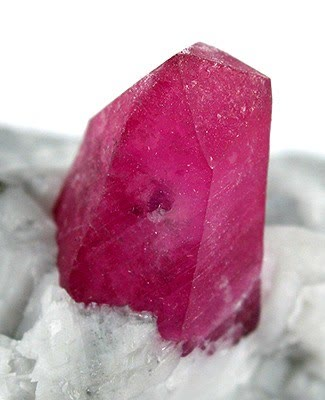
\includegraphics[height=4.2cm]{images/book4/ruby-crystal.jpg}\par
{\small rubi}
\end{minipage}\hspace{1.5em}
\begin{minipage}[b]{0.3\linewidth}\centering
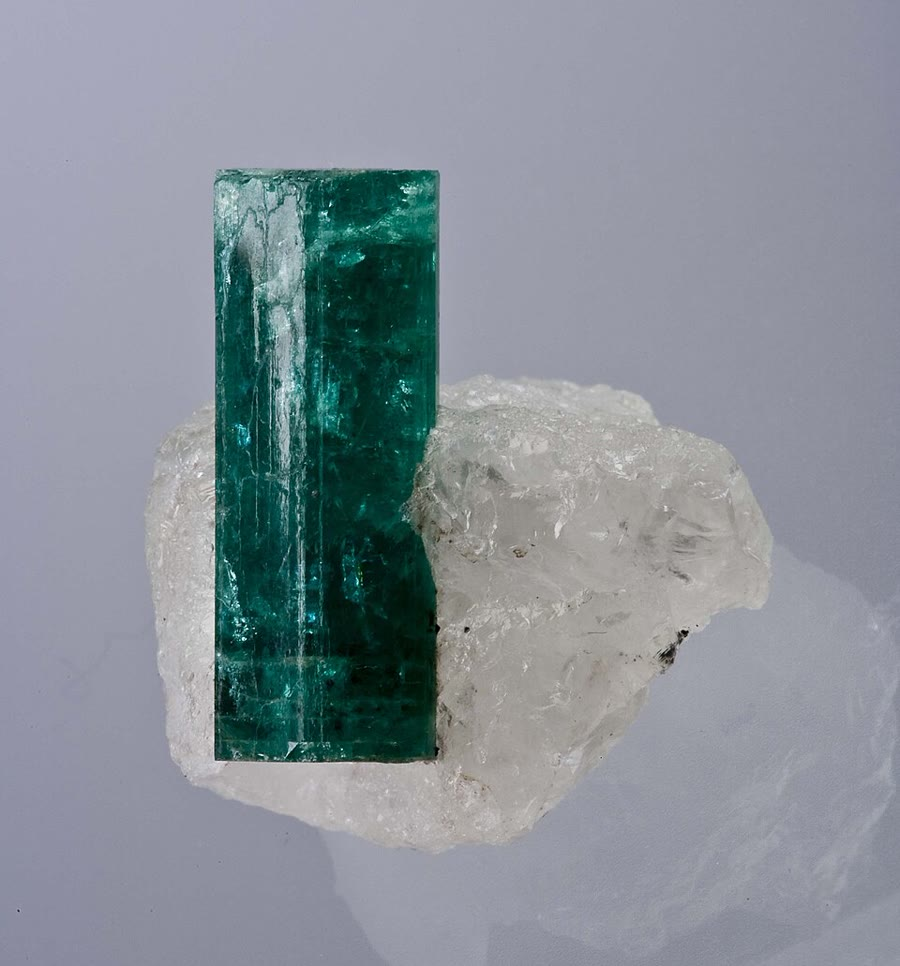
\includegraphics[height=4.2cm]{images/book4/emerald-crystal.jpg}\par
{\small zamrud}
\end{minipage}

{\small Kristal rubi dalam marmer dan kristal zamrud pada kuarsa. Pada keduanya,
warna berasal dari beberapa persen \ce{Cr^{3+}} di sebuah situs oktahedral.}
\end{omfigure}

\section{Dari suku ion bebas ke suku medan ligan}

Pada ion bebas, tolakan elektron memecah konfigurasi $d^n$ menjadi suku-suku
($^4$F, $^4$P, $^2$G\dots\ untuk $d^3$, \cref{ch:b3:many-electron-atoms}). Dalam kompleks, setiap suku
dipecah lebih lanjut oleh ligan, dan tingkat-tingkatnya diberi label dengan
\omterm{def:b3:point-groups:irrep}{representasi tak tereduksi} \omterm{def:b3:point-groups:point-group}{grup titik} kompleks itu.

\begin{definition}[Suku medan ligan]\label{def:b3:complex-spectra-magnetism:ligand-field-term}
Yang disebut \emph{suku medan ligan}\index{suku medan ligan} sebuah kompleks adalah himpunan
keadaan banyak-elektron yang terdegenerasi, yang diberi label dengan
\omterm{def:b3:many-electron-atoms:term}{multiplisitas spinnya} dan dengan \omterm{def:b3:point-groups:irrep}{representasi tak tereduksi} \omterm{def:b3:point-groups:point-group}{grup titik} tempat
bagian orbitalnya berada, misalnya $^4$A$_{2g}$ atau $^4$T$_{1g}$ dalam kompleks oktahedral.
\end{definition}

\begin{proposition}[Karakter grup rotasi]\label{prop:b3:complex-spectra-magnetism:rotation-characters}
Ke-$2L+1$ keadaan sebuah suku dengan momentum sudut orbital $L$ membentuk
representasi rotasi-rotasi yang \omterm{def:b3:point-groups:representation}{karakternya} untuk rotasi sebesar $\alpha$ adalah
\[
  \chi_L(\alpha) = \frac{\sin\bigl((L + \tfrac12)\alpha\bigr)}{\sin(\alpha/2)}, \qquad \chi_L(0) = 2L + 1 .
\]
\end{proposition}

\admitted

\begin{theorem}[Pembelahan suku ion bebas dalam medan oktahedral]\label{thm:b3:complex-spectra-magnetism:term-splitting}
Dalam medan oktahedral, suku-suku ion $d^n$ terpecah menjadi
\begin{center}
\begin{tabular}{ll}
\hline
suku ion bebas & suku oktahedral (\omterm{def:b3:many-electron-atoms:term}{multiplisitas spin} sama) \\ \hline
S & A$_{1g}$ \\
P & T$_{1g}$ \\
D & E$_g$ + T$_{2g}$ \\
F & A$_{2g}$ + T$_{1g}$ + T$_{2g}$ \\
G & A$_{1g}$ + E$_g$ + T$_{1g}$ + T$_{2g}$ \\ \hline
\end{tabular}
\end{center}
\end{theorem}

\begin{proof}
Grup oktahedral adalah grup rotasi $O$ kali inversi; fungsi-fungsi $d$
bersifat genap, sehingga setiap suku konfigurasi $d^n$ genap ($g$), dan cukuplah
mereduksi dalam $O$, yang kelas-kelasnya adalah $E$, $8C_3$, $3C_2$ ($=C_4^2$), $6C_4$, dan $6C_2'$. Dengan
proposisi itu, untuk $L = 3$: $\chi = 7$, $\sin(420^\circ)/\sin60^\circ = 1$, $\sin(630^\circ)/\sin90^\circ = -1$, $\sin(315^\circ)/\sin45^\circ = -1$,
dan $-1$. \omterm{def:b3:point-groups:irrep}{Tabel karakter} $O$ (baris $A_1$: 1, 1, 1, 1, 1; $A_2$: 1, 1, 1, $-1$, $-1$; $E$: 2,
$-1$, 2, 0, 0; $T_1$: 3, 0, $-1$, 1, $-1$; $T_2$: 3, 0, $-1$, $-1$, 1) dan \omterm{thm:b3:group-theory-applied:reduction}{rumus reduksi} pada
\cref{ch:b3:group-theory-applied} memberikan $n(A_2) = (7 + 8 - 3 + 6 + 6)/24 = 1$, $n(T_1) = (21 + 3 - 6 +
6)/24 = 1$, $n(T_2) = (21 + 3 + 6 - 6)/24 = 1$, dan nol untuk $A_1$ dan $E$. Baris-baris lainnya
diperoleh dengan cara yang sama ($L = 0$: $(1, 1, 1, 1, 1)$; $L = 1$: $(3, 0, -1, 1, -1)$; $L = 2$: $(5, -1, 1,
-1, 1)$; $L = 4$: $(9, 0, 1, 1, 1)$).
\end{proof}

\begin{method}[Memecah suku ion bebas]\label{met:b3:complex-spectra-magnetism:split-term}
\begin{enumerate}
  \item Tentukan suku dasar ion bebas (aturan Hund) dan suku-suku tereksitasi
        yang multiplisitasnya sama.
  \item Bacalah komponen-komponen oktahedralnya pada tabel; \omterm{def:b3:many-electron-atoms:term}{multiplisitas spinnya}
        tidak berubah.
  \item Urutkan komponen-komponen itu: untuk suku dasar F pada $d^2$, $d^7$ (spin tinggi), yang terendah adalah T$_{1g}$;
        untuk $d^3$, $d^8$, yang terendah adalah A$_{2g}$ (proposisi berikut).
\end{enumerate}
\end{method}

\begin{proposition}[Lubang dan pembalikan tetrahedral]\label{prop:b3:complex-spectra-magnetism:hole}
Suku-suku $d^{10-n}$ dalam medan oktahedral adalah suku-suku $d^n$ dengan urutan energi
terbalik; suku-suku $d^n$ dalam medan tetrahedral adalah suku-suku $d^{10-n}$ dalam medan
oktahedral (dengan subskrip $g$ dihilangkan).
\end{proposition}

\begin{proof}
Konfigurasi $d^{10-n}$ setara dengan $n$ lubang positif dalam kulit yang penuh:
lubang-lubang itu merasakan potensial medan ligan dengan tanda yang berlawanan,
sehingga setiap pembelahan satu-elektron, dan karena itu setiap pembelahan
suku, terbalik (tolakan elektron antara lubang sama dengan tolakan antara
elektron). Medan tetrahedral bertanda berlawanan dengan medan oktahedral
(orbital $e$ terletak lebih rendah) dan tidak memiliki pusat simetri: $d^n$ dalam $T_d$ berperilaku seperti $d^n$ dengan
medan terbalik, yaitu seperti $d^{10-n}$ dalam $O_h$.
\end{proof}

\begin{definition}[Diagram korelasi]\label{def:b3:complex-spectra-magnetism:correlation}
Yang disebut \emph{diagram korelasi}\index{diagram korelasi} adalah diagram yang
menghubungkan keadaan-keadaan sebuah sistem dalam dua situasi limit, di sini
suku-suku ion bebas yang dipecah oleh medan lemah dan konfigurasi-konfigurasi $t_{2g}^ae_g^b$
medan kuat, dengan menghubungkan keadaan-keadaan yang simetrinya sama tanpa
membiarkan dua di antaranya bersilangan.
\end{definition}

\begin{omfigure}
\begin{tikzpicture}[font=\small]
  % ion bebas
  \pic (F) at (0,0) {omlevel={}{1.1}};
  \pic (P) at (0,3.0) {omlevel={}{1.1}};
  \node[anchor=east] at (F-l) {$^3$F};
  \node[anchor=east] at (P-l) {$^3$P};
  % medan lemah
  \pic (a) at (2.6,-0.8) {omlevel={}{1.0}};
  \pic (b) at (2.6,0.3) {omlevel={}{1.0}};
  \pic (c) at (2.6,1.4) {omlevel={}{1.0}};
  \pic (d) at (2.6,3.1) {omlevel={}{1.0}};
  \foreach \n/\t in {a/T$_{1g}$, b/T$_{2g}$, c/A$_{2g}$, d/T$_{1g}$(P)}{\node[omsymlabel, anchor=south] at (\n-c) {$^3$\t};}
  \draw[omcorr] (F-r) -- (a-l) (F-r) -- (b-l) (F-r) -- (c-l) (P-r) -- (d-l);
  % konfigurasi medan kuat
  \pic (A) at (7.4,-1.6) {omlevel={}{1.0}};
  \pic (B) at (7.4,1.4) {omlevel={}{1.0}};
  \pic (C) at (7.4,1.9) {omlevel={}{1.0}};
  \pic (D) at (7.4,4.6) {omlevel={}{1.0}};
  \node[anchor=west] at (A-r) {$^3$T$_{1g}$ \quad $t_{2g}^2$};
  \node[anchor=west] at (B-r) {$^3$T$_{2g}$};
  \node[anchor=west] at (C-r) {$^3$T$_{1g}$ \quad $t_{2g}e_g$};
  \node[anchor=west] at (D-r) {$^3$A$_{2g}$ \quad $e_g^2$};
  \draw[omcorr] (a-r) -- (A-l) (b-r) -- (B-l) (c-r) -- (D-l) (d-r) -- (C-l);
  \node[anchor=north] at (0,-2.0) {ion bebas};
  \node[anchor=north] at (2.6,-2.0) {medan lemah};
  \node[anchor=north] at (7.4,-2.0) {medan kuat};
  \draw[->, black!50] (3.7,-2.3) -- (6.2,-2.3) node[midway, below, font=\scriptsize] {$\Delta_{\mathrm o}$ bertambah};
\end{tikzpicture}

{\small \omterm{def:b3:complex-spectra-magnetism:correlation}{Diagram korelasi} \omterm{def:b3:many-electron-atoms:singlet-triplet}{keadaan-keadaan triplet} ion $d^2$ dalam medan
oktahedral. Setiap suku medan lemah menuju konfigurasi medan kuat yang
simetrinya sama, dan kedua keadaan $^3$T$_{1g}$ tidak bersilangan: yang lebih rendah menuju $t_{2g}^2$, yang lebih tinggi menuju
$t_{2g}e_g$.}
\end{omfigure}

\section{Diagram Tanabe--Sugano}

\begin{definition}[Parameter Racah]\label{def:b3:complex-spectra-magnetism:racah}
Yang disebut \emph{parameter Racah}\index{parameter Racah} $A$, $B$, dan $C$ adalah kombinasi
integral-integral Slater kulit $d$ yang menyatakan semua energi tolakan
elektron sebuah konfigurasi $d^n$; selisih energi antara suku-suku konfigurasi
yang sama hanya bergantung pada $B$ dan $C$, dan selisih antara suku-suku yang
multiplisitasnya sama-sama tertinggi hanya bergantung pada $B$ (untuk $d^2$, $d^3$, $d^7$, $d^8$: $E(\mathrm P) - E(\mathrm F) = 15B$).
\end{definition}

\begin{example}[Parameter Racah ion bebas]\label{ex:b3:complex-spectra-magnetism:free-B}
% ledger: lev:Cr3.4F5_2, lev:Cr3.4F7_2, lev:Cr3.4F9_2, lev:Cr3.4P1_2, lev:Cr3.4P3_2, lev:Cr3.4P5_2, lev:Ni2.3F3, lev:Ni2.3F2, lev:Ni2.3P2, lev:Ni2.3P1, lev:Ni2.3P0, lev:V2.4F5_2, lev:V2.4F7_2, lev:V2.4F9_2, lev:V2.4P1_2, lev:V2.4P3_2, lev:V2.4P5_2
Tingkat-tingkat ion \ce{Cr^{3+}} bebas menempatkan pusat berat (dengan bobot $2J + 1$) $^4$F pada
\qty{547}{cm^{-1}} dan pusat berat $^4$P pada \qty{14305}{cm^{-1}} di atas tingkat dasar: $15B = \qty{13758}{cm^{-1}}$,
$B = \qty{917}{cm^{-1}}$. Perhitungan yang sama memberikan $B = 755$ untuk \ce{V^{2+}} dan \qty{1056}{cm^{-1}} untuk
\ce{Ni^{2+}}.
\end{example}

\begin{definition}[Diagram Tanabe--Sugano]\label{def:b3:complex-spectra-magnetism:tanabe-sugano}
Yang disebut \emph{diagram Tanabe--Sugano}\index{diagram Tanabe--Sugano} adalah alur energi
semua \omterm{def:b3:complex-spectra-magnetism:ligand-field-term}{suku medan ligan} sebuah ion $d^n$, dalam satuan $B$ dan diukur dari
suku dasar, terhadap $\Delta_{\mathrm o}/B$, untuk rasio $C/B$ yang tetap.
\end{definition}

\begin{proposition}[Tiga pita ion $d^3$]\label{prop:b3:complex-spectra-magnetism:d3-bands}
Untuk ion $d^3$ dalam medan oktahedral, transisi yang diizinkan spin dari $^4$A$_{2g}$ terletak pada
\[
  \nu_1 = \Delta_{\mathrm o}\ (^4\mathrm T_{2g}), \qquad
  \nu_{2,3} = 7.5B + 1.5\Delta_{\mathrm o} \mp \tfrac12\sqrt{225B^2 - 18B\Delta_{\mathrm o} + \Delta_{\mathrm o}^2}\ (^4\mathrm T_{1g}(\mathrm F), {}^4\mathrm T_{1g}(\mathrm P)).
\]
\end{proposition}

\begin{proof}[Bukti parsial]
Dalam basis medan kuat, $^4$A$_{2g}$ dan $^4$T$_{2g}$ masing-masing muncul satu kali, dari $t_{2g}^3$ dan $t_{2g}^2e_g$, dan
selisih keduanya tidak mengandung tolakan elektron: $\nu_1 = \Delta_{\mathrm o}$ secara eksak. $^4$T$_{1g}$ muncul
dua kali, dari $t_{2g}^2e_g$ dan $t_{2g}e_g^2$; relatif terhadap $^4$A$_{2g}$, matriks $2\times2$-nya adalah
$\begin{pmatrix}\Delta_{\mathrm o} + 12B & 6B\\ 6B & 2\Delta_{\mathrm o} + 3B\end{pmatrix}$ (unsur-unsur tolakan elektronnya diterima tanpa bukti).
\omterm{def:b3:quantum-model-systems:operator}{Nilai-nilai eigennya} adalah akar-akar $E^2 - (15B + 3\Delta_{\mathrm o})E + 2\Delta_{\mathrm o}^2 + 27B\Delta_{\mathrm o} = 0$, yaitu
$\nu_2$ dan $\nu_3$ yang dinyatakan di atas. Pada $\Delta_{\mathrm o} = 0$ nilainya 0 dan $15B$ (suku $^4$F dan $^4$P); diagonalisasi
lengkap pada gambar mereproduksinya.
\end{proof}

\begin{omfigure}
\begin{tikzpicture}
\begin{axis}[name=ta, omts, width=0.46\linewidth, height=7.0cm, xmin=1, xmax=40, ymin=0, ymax=70,
  xlabel={$\Delta_{\mathrm o}/B$}, ylabel={$E/B$}, title={\small $d^3$, $C/B = 4.5$},
  unbounded coords=jump, clip=true, clip mode=individual]
\foreach \c in {f0,f1,f2,f3,f4,f5,f6,f7,f8,f9,f10,f11,f12,f13,f14,f15}{
  \addplot[omtsforbidden, restrict x to domain=1:40] table[x=x, y=\c] {figdata/out/bachelor-3-tanabe-sugano-d3.dat};}
\foreach \c in {a0,a1,a2,a3}{
  \addplot[omDef, thick, restrict x to domain=1:40] table[x=x, y=\c] {figdata/out/bachelor-3-tanabe-sugano-d3.dat};}
\draw[omThm, dashed] (axis cs:29.0,0) -- (axis cs:29.0,70);
\draw[black!70, dashed] (axis cs:27.1,0) -- (axis cs:27.1,70);
\node[font=\scriptsize, omThm, anchor=north west, rotate=90] at (axis cs:29.6,1.5) {rubi};
\node[font=\scriptsize, anchor=south west, rotate=90] at (axis cs:26.6,1.5) {zamrud};
% label di luar bingkai, pada ketinggian tempat setiap kurva meninggalkannya
\node[font=\scriptsize, omDef, anchor=west, inner sep=1pt] at (axis cs:40,40) {$^4$T$_{2g}$};
\node[font=\scriptsize, omDef, anchor=west, inner sep=1pt] at (axis cs:40,50.9) {$^4$T$_{1g}$};
\node[font=\scriptsize, omDef, anchor=south, inner sep=1pt] at (axis cs:32.8,70) {$^4$T$_{1g}$(P)};
\node[font=\scriptsize, black!60, anchor=west, inner sep=1pt] at (axis cs:40,21.2) {$^2$E$_g$};
\end{axis}
\begin{axis}[at={(ta.east)}, anchor=west, xshift=2.2cm, omts, width=0.46\linewidth, height=7.0cm,
  xmin=1, xmax=40, ymin=0, ymax=70, xlabel={$\Delta_{\mathrm o}/B$}, ylabel={$E/B$},
  title={\small $d^8$, $C/B = 4.71$}, unbounded coords=jump, clip=true, clip mode=individual]
\foreach \c in {f0,f1,f2,f3,f4,f5,f6}{
  \addplot[omtsforbidden, restrict x to domain=1:40] table[x=x, y=\c] {figdata/out/bachelor-3-tanabe-sugano-d8.dat};}
\foreach \c in {a0,a1,a2,a3}{
  \addplot[omDef, thick, restrict x to domain=1:40] table[x=x, y=\c] {figdata/out/bachelor-3-tanabe-sugano-d8.dat};}
\node[font=\scriptsize, omDef, anchor=west, inner sep=1pt] at (axis cs:40,40) {$^3$T$_{2g}$};
\node[font=\scriptsize, omDef, anchor=west, inner sep=1pt] at (axis cs:40,50.9) {$^3$T$_{1g}$};
\node[font=\scriptsize, omDef, anchor=south, inner sep=1pt] at (axis cs:32.8,70) {$^3$T$_{1g}$(P)};
\end{axis}
\end{tikzpicture}

{\small \omterm{def:b3:complex-spectra-magnetism:tanabe-sugano}{Diagram Tanabe--Sugano} ion $d^3$ dan $d^8$ yang dihitung dengan mendiagonalisasi
Hamiltonian medan ligan dan tolakan elektron atas semua keadaan
konfigurasinya. Biru tebal: keadaan-keadaan dengan multiplisitas keadaan dasar
(transisi yang diizinkan spin); abu-abu tipis: keadaan-keadaan lainnya. Suku dasarnya adalah
sumbu mendatar ($^4$A$_{2g}$ untuk $d^3$, $^3$A$_{2g}$ untuk $d^8$). Putus-putus: rubi dan zamrud, yang ditempatkan pada $\Delta_{\mathrm o}/B$ kedua pitanya.
Tingkat $^2$E$_g$ pada $d^3$ hampir datar: energinya nyaris tidak bergantung pada medan.}
\end{omfigure}

\begin{method}[Membaca diagram Tanabe--Sugano]\label{met:b3:complex-spectra-magnetism:read-ts}
\begin{enumerate}
  \item Kenali suku dasar dan transisi-transisi yang diizinkan spin (yang
        multiplisitasnya sama).
  \item Hitunglah rasio energi dua pita, $\nu_2/\nu_1$; carilah nilai $\Delta_{\mathrm o}/B$ yang
        membuat diagram memberikan rasio itu.
  \item Bacalah $E/B$ untuk $\nu_1$ di situ: $B = \nu_1/(E/B)$, lalu $\Delta_{\mathrm o}$. Untuk $d^3$ dan $d^8$, $\Delta_{\mathrm o} = \nu_1$
        secara langsung dan rumus tertutupnya memberikan $B$ dari $\nu_2$.
  \item Bandingkan $B$ dengan nilai ion bebas (\omterm{def:b3:complex-spectra-magnetism:nephelauxetic}{rasio nefelauksetik}) dan periksalah bahwa
        pita ketiga jatuh di tempat yang diramalkan diagram.
\end{enumerate}
\end{method}

\begin{definition}[Efek nefelauksetik]\label{def:b3:complex-spectra-magnetism:nephelauxetic}
Yang disebut \emph{efek nefelauksetik}\index{efek nefelauksetik} (``pengembang awan'') adalah
penurunan \omterm{def:b3:complex-spectra-magnetism:racah}{parameter Racah} $B$ sebuah ion logam dalam kompleks dibandingkan dengan
ion bebasnya, yang disebabkan oleh delokalisasi elektron $d$ ke
ligan; \emph{rasio nefelauksetik}\index{rasio nefelauksetik} adalah $\beta =
B_{\text{kompleks}}/B_{\text{ion bebas}}$.
\end{definition}

Ligan yang berikatan secara lebih kovalen lebih banyak menurunkan $B$: $\beta$ mendekati 0.9 untuk fluorida, 0.8
untuk air, 0.6 sampai 0.7 untuk oksida dan halida yang lebih berat, dan lebih
rendah lagi untuk sulfida. Transisi terlarang spin, antara suku-suku yang
multiplisitasnya berbeda, muncul sebagai garis yang lemah dan sering tajam.

\section{Intensitas dan transfer muatan}

\begin{definition}[Kopling vibronik]\label{def:b3:complex-spectra-magnetism:vibronic-coupling}
Yang disebut \emph{kopling vibronik}\index{kopling vibronik} adalah pencampuran gerak elektronik
dan gerak vibrasi: vibrasi asimetris yang menghilangkan pusat simetri sebuah
kompleks mencampurkan sedikit karakter ganjil ($u$) ke dalam keadaan-keadaan $d$-nya,
sehingga transisi $d$--$d$ yang terlarang Laporte menjadi sedikit diizinkan.
\end{definition}

\begin{proposition}[Intensitas pita serapan]\label{prop:b3:complex-spectra-magnetism:intensity-order}
Koefisien serapan molar pita-pita kompleks bertambah dalam urutan berikut:
$d$--$d$ terlarang spin $\ll$ $d$--$d$ diizinkan spin dalam kompleks sentrosimetris $<$ $d$--$d$
dalam kompleks tetrahedral $<$ transfer muatan.
\end{proposition}

\begin{proof}[Argumen]
Menurut \cref{ch:b3:electronic-spectroscopy}, sebuah transisi diizinkan jika spin
kekal dan paritasnya berubah. Transisi $d$--$d$ tidak pernah mengubah paritas: dalam
kompleks oktahedral, transisi itu meminjam intensitas hanya melalui \omterm{def:b3:complex-spectra-magnetism:vibronic-coupling}{kopling vibronik}; dalam
tetrahedron, yang tidak memiliki pusat simetri, orbital $d$ dan $p$ tercampur secara permanen.
Transisi terlarang spin meminjam satu fraksi kecil lagi melalui \omterm{def:b3:many-electron-atoms:spin-orbit}{kopling
spin--orbit}. \omterm{def:b3:electronic-spectroscopy:charge-transfer}{Transisi transfer muatan} memindahkan elektron antara
orbital-orbital yang paritasnya berbeda pada logam dan ligan, dan sepenuhnya
diizinkan.
\end{proof}

\begin{definition}[Transfer muatan]\label{def:b3:complex-spectra-magnetism:ct}
Dalam \emph{transfer muatan ligan-ke-logam}\index{transfer muatan ligan-ke-logam}
(LMCT), sebuah elektron berpindah dari orbital yang berpusat pada ligan ke orbital
yang berpusat pada logam; dalam \emph{transfer muatan logam-ke-ligan}\index{transfer muatan logam-ke-ligan}
(MLCT), elektron berpindah dari logam ke orbital $\pi^*$ ligan.
\end{definition}

Permanganat dan kromat, ion $d^0$ yang sama sekali tidak memiliki transisi $d$--$d$, berwarna
pekat karena LMCT dari oksida ke orbital $d$ logam yang kosong, yang mudah terjadi pada logam
berbilangan oksidasi tinggi. $\ce{[Ru(bpy)3]^{2+}}$ (bpy: 2,2$'$-bipiridina) berwarna jingga karena MLCT
dari rutenium(II) ke orbital-orbital $\pi^*$ ligannya, yaitu keadaan tereksitasi yang dipakai dalam
\omterm{def:b3:photochemistry:photoredox}{katalisis fotoredoks} (\cref{ch:b3:photochemistry}). Pada rubi, kedua pita lebar
di dekat 560 dan \qty{410}{nm} adalah pita $d$--$d$ yang diizinkan spin pada
\cref{prop:b3:complex-spectra-magnetism:d3-bands}; cahaya yang diteruskan berwarna merah,
dengan sedikit biru. Setelah tereksitasi ke dalam pita-pita ini, ion itu berelaksasi ke tingkat $^2$E$_g$ dan
dari situ memancarkan garis R merah tua di dekat \qty{695}{nm}, yaitu garis laser yang pertama.

\section{Efek Jahn--Teller}

\begin{theorem}[Teorema Jahn--Teller]\label{thm:b3:complex-spectra-magnetism:jahn-teller}
Molekul tak linear dalam keadaan elektronik yang terdegenerasi secara orbital tidak
stabil terhadap distorsi yang menurunkan simetrinya dan menghilangkan
\omterm{def:b3:quantum-model-systems:degenerate}{degenerasinya}. Inilah \emph{teorema Jahn--Teller}\index{teorema Jahn--Teller}.
\end{theorem}

\admitted

Akibat-akibatnya bagi kompleks oktahedral mengikuti dari pengisian orbital
$e_g$, yang mengarah ke ligan. Pada ion $d^9$ (\ce{Cu^{2+}}), konfigurasi
$t_{2g}^6e_g^3$ memiliki lubang di $d_{z^2}$ atau di $d_{x^2-y^2}$: sebuah keadaan E$_g$. Meregangkan kedua ikatan aksial
menurunkan $d_{z^2}$ dan menaikkan $d_{x^2-y^2}$; menempatkan dua elektron di orbital yang diturunkan
dan satu di orbital yang dinaikkan memberikan stabilisasi neto. Kompleks tembaga(II)
memang berupa oktahedron yang memanjang, dengan empat ikatan pendek dan dua ikatan panjang. Hal yang sama berlaku
untuk $d^4$ spin tinggi (\ce{Mn^{3+}}, \ce{Cr^{2+}}) dan $d^7$ spin rendah; untuk himpunan $t_{2g}$ yang terisi tidak merata
($d^1$, $d^2$, $d^5$ spin rendah\dots), orbital-orbitalnya mengarah di antara ligan dan
distorsinya kecil. Keadaan tereksitasi kompleks yang terdegenerasi juga terdistorsi: pita-pita
\ce{[Ti(H2O)6]^{3+}} dan kompleks tembaga(II) yang lebar dan sering berpunuk ganda merupakan
tanda spektroskopiknya.

\begin{omfigure}
\begin{tikzpicture}[font=\small]
  \pic[transform shape] (t) at (0,0) {omlevel={}{1.6}};
  \pic[transform shape] (e) at (0,2.2) {omlevel={}{1.1}};
  \node[anchor=east] at (t-l) {$t_{2g}$};
  \node[anchor=east] at (e-l) {$e_g$};
  \pic[transform shape] (xy) at (4.2,0.45) {omlevel={ud}{0.8}};
  \pic[transform shape] (xz) at (4.2,-0.25) {omlevel={ud}{1.4}};
  \pic[transform shape] (x2) at (4.2,3.0) {omlevel={u}{0.8}};
  \pic[transform shape] (z2) at (4.2,1.5) {omlevel={ud}{0.8}};
  \draw[omcorr] (t-r) -- (xy-l) (t-r) -- (xz-l) (e-r) -- (x2-l) (e-r) -- (z2-l);
  \node[anchor=west] at (xy-r) {$b_{2g}$ ($d_{xy}$)};
  \node[anchor=west] at (xz-r) {$e_g$ ($d_{xz}$, $d_{yz}$)};
  \node[anchor=west] at (x2-r) {$b_{1g}$ ($d_{x^2-y^2}$)};
  \node[anchor=west] at (z2-r) {$a_{1g}$ ($d_{z^2}$)};
  \node[anchor=north] at (0,-0.9) {$O_h$};
  \node[anchor=north] at (4.2,-0.9) {$D_{4h}$, memanjang};
  \begin{scope}[xshift=9.0cm, yshift=1.2cm, scale=0.8]
    \pic[transform shape] {omoctahedron};
    \draw[->, thick, omThm] (0,1.25) -- (0,1.85);
    \draw[->, thick, omThm] (0,-1.25) -- (0,-1.85);
  \end{scope}
\end{tikzpicture}

{\small Distorsi Jahn--Teller kompleks oktahedral $d^9$: meregangkan ikatan-ikatan aksial (kanan) memecah $e_g$ menjadi $a_{1g}$
($d_{z^2}$, diturunkan) dan $b_{1g}$ ($d_{x^2-y^2}$, dinaikkan), dan $t_{2g}$ menjadi $e_g$ dan $b_{2g}$. Dengan sembilan
elektron, satu-satunya lubang menempati $b_{1g}$: distorsi itu merupakan stabilisasi neto.}
\end{omfigure}

\section{Kemagnetan}

\begin{definition}[Suseptibilitas magnetik]\label{def:b3:complex-spectra-magnetism:susceptibility}
Yang disebut \emph{suseptibilitas magnetik}\index{suseptibilitas magnetik} $\chi$ sebuah bahan
adalah rasio magnetisasinya terhadap kuat medan yang diberikan; \emph{suseptibilitas
molar}\index{suseptibilitas molar} $\chi_{\mathrm m}$ adalah suseptibilitas per mol.
Zat paramagnetik memiliki $\chi > 0$, zat diamagnetik $\chi < 0$ yang kecil. Para kimiawan sering
memakai nilai cgs $\chi_{\mathrm m}$, dalam \unit{cm^3.mol^{-1}}, yang sama dengan nilai SI dalam \unit{m^3.mol^{-1}}
dibagi dengan $4\pi\times10^{-6}$.
\end{definition}

\begin{definition}[Tetapan Curie]\label{def:b3:complex-spectra-magnetism:curie}
Yang disebut \emph{tetapan Curie}\index{tetapan Curie} $C$ sebuah paramagnet yang mematuhi
\omterm{thm:b3:complex-spectra-magnetism:curie}{hukum Curie} adalah hasil kali $\chi_{\mathrm m}T$.
\end{definition}

\begin{theorem}[Hukum Curie]\label{thm:b3:complex-spectra-magnetism:curie}
Untuk spin-spin $S$ yang saling bebas dengan faktor $g$ sebesar $g$, pada suhu-suhu yang memenuhi $g\mu_BB \ll kT$,
\[
  \chi_{\mathrm m} = \frac{C}{T}, \qquad C = \frac{\mu_0N_Ag^2\mu_B^2S(S+1)}{3k}\ \ (\text{SI});
\]
dalam satuan cgs $C = 0.1251\,g^2S(S+1)$ \unit{cm^3.K.mol^{-1}}. Inilah \emph{hukum Curie}\index{hukum Curie}.
\end{theorem}

\begin{proof}[Bukti parsial]
Untuk $S = \frac12$, kedua tingkat $m_S = \pm\frac12$ memiliki energi $\pm\frac12g\mu_BB$ dalam medan $B$. Menurut
\omterm{def:b3:partition-functions:boltzmann}{distribusi Boltzmann}, momen rata-rata searah medan adalah $\frac12g\mu_B\tanh(g\mu_BB/2kT) \approx
g^2\mu_B^2B/4kT$; per mol, $M = N_Ag^2\mu_B^2B/4kT$, dan dengan $\chi_{\mathrm m} = \mu_0M/B$, $\chi_{\mathrm m} = \mu_0N_Ag^2\mu_B^2/(4kT)$,
yang merupakan rumus itu dengan $S(S+1) = \frac34$. Kasus umumnya (merata-ratakan $m_S^2$ atas $2S + 1$
tingkat, $\langle m_S^2\rangle = S(S+1)/3$) diterima tanpa bukti.
\end{proof}

\begin{definition}[Momen magnetik efektif]\label{def:b3:complex-spectra-magnetism:moment}
Yang disebut \emph{momen magnetik efektif}\index{momen magnetik efektif} sebuah
ion paramagnetik adalah $\mu_{\mathrm{eff}} = \sqrt{3k\chi_{\mathrm m}T/(\mu_0N_A)}$, dalam cgs $\mu_{\mathrm{eff}}/\mu_B = 2.828\sqrt{\chi_{\mathrm m}T}$.
Yang disebut \emph{momen spin saja}\index{momen spin saja} ion itu adalah nilai $2\sqrt{S(S+1)}\,\mu_B$ yang
akan diberikan oleh spin-spinnya saja dengan $g = 2$; kelebihan momen terukur di atas nilai itu
disebut \emph{kontribusi orbital}\index{kontribusi orbital}.
\end{definition}

\begin{proposition}[Rumus spin saja]\label{prop:b3:complex-spectra-magnetism:spin-only}
Untuk $n$ elektron yang tidak berpasangan, $\mu_{\text{spin saja}} = \sqrt{n(n+2)}\,\mu_B$: 1.73, 2.83, 3.87, 4.90, dan $5.92\,\mu_B$ untuk
$n = 1$ sampai 5.
\end{proposition}

\begin{proof}
$S = n/2$, sehingga $2\sqrt{S(S+1)} = 2\sqrt{\frac n2(\frac n2 + 1)} = \sqrt{n(n+2)}$.
\end{proof}

\begin{proposition}[Kontribusi orbital]\label{prop:b3:complex-spectra-magnetism:orbital-contribution}
Dalam kompleks oktahedral, ion-ion dengan suku dasar A atau E memiliki momen yang dekat dengan
nilai spin saja; ion-ion dengan suku dasar T dapat memiliki \omterm{def:b3:complex-spectra-magnetism:moment}{kontribusi orbital}
yang cukup besar.
\end{proposition}

\begin{proof}[Argumen]
Momen orbital memerlukan sebuah orbital yang dapat diubah menjadi orbital lain
yang setara dan terdegenerasi melalui rotasi terhadap sumbu medan, dengan
sebuah elektron yang bebas berpindah di antara keduanya. Dalam keadaan T (himpunan $t_{2g}$ terisi tidak merata), orbital-orbital $d_{xz}$, $d_{yz}$, $d_{xy}$
saling terkait melalui rotasi $90^\circ$ dan momennya bertahan sebagian; dalam keadaan A dan E
($t_{2g}^3$, $t_{2g}^6e_g^2$, $e_g$ terisi sebagian) tidak tersedia orbital setara semacam itu dan
momen orbitalnya terpadamkan.
\end{proof}

\begin{definition}[Transisi spin]\label{def:b3:complex-spectra-magnetism:spin-crossover}
Yang disebut \emph{transisi spin}\index{transisi spin} adalah perubahan sebuah kompleks
antara keadaan spin rendah dan keadaan spin tinggi oleh suhu, tekanan, atau cahaya,
yang mungkin terjadi jika $\Delta_{\mathrm o}$ dekat dengan energi pemasangan.
\end{definition}

\begin{proposition}[Suhu transisi]\label{prop:b3:complex-spectra-magnetism:crossover}
Jika perubahan $\mathrm{LS} \rightleftharpoons \mathrm{HS}$ berperilaku sebagai kesetimbangan dengan entalpi $\Delta H$ dan entropi $\Delta S$,
fraksi spin tingginya adalah $x_{\mathrm{HS}} = 1/(1 + \eu^{(\Delta H - T\Delta S)/RT})$, yang bernilai setengah pada $T_{1/2} = \Delta H/\Delta S$.
\end{proposition}

\begin{proof}
$K = x_{\mathrm{HS}}/(1 - x_{\mathrm{HS}}) = \eu^{-(\Delta H - T\Delta S)/RT}$; $K = 1$ ketika $\Delta H = T\Delta S$.
\end{proof}

Baik $\Delta H$ maupun $\Delta S$ bernilai positif: keadaan spin tinggi memiliki ikatan logam--ligan
yang lebih panjang dan lebih lemah serta lebih banyak keadaan spin ($R\ln5$ dari spin saja untuk besi(II), $S = 2$),
sehingga keadaan itu menang pada suhu tinggi.

\begin{omfigure}
\begin{tikzpicture}
\begin{axis}[name=ct, width=0.47\linewidth, height=5.2cm, xmin=0, xmax=400, ymin=0, ymax=5.6,
  axis lines=left, xlabel={$T$ / K}, ylabel={$\chi_{\mathrm m}T$ / \unit{cm^3.K.mol^{-1}}},
  tick label style={font=\small}, label style={font=\small}]
\addplot[omDef, thick] table[x=T, y=chiT_para] {figdata/out/bachelor-3-curie-chiT.dat};
\addplot[omThm, thick] table[x=T, y=chiT_sco] {figdata/out/bachelor-3-curie-chiT.dat};
\node[font=\scriptsize, omDef, anchor=south west] at (axis cs:20,4.45) {paramagnet Curie, $S = \frac52$};
\node[font=\scriptsize, omThm, anchor=west, align=left] at (axis cs:20,2.4) {transisi spin,\\ $T_{1/2} = \qty{200}{K}$};
\end{axis}
\begin{axis}[at={(ct.east)}, anchor=west, xshift=1.5cm, width=0.47\linewidth, height=5.2cm,
  xmin=0, xmax=100, ymin=0, ymax=0.46, axis lines=left, xlabel={$1000\,\mathrm K/T$},
  ylabel={$\chi_{\mathrm m}$ / \unit{cm^3.mol^{-1}}}, tick label style={font=\small},
  label style={font=\small}]
\addplot[omDef, thick] table[x=invT, y=chi] {figdata/out/bachelor-3-curie-chi.dat};
\end{axis}
\end{tikzpicture}

{\small Kiri: $\chi_{\mathrm m}T$ terhadap $T$ untuk paramagnet Curie ($S = \frac52$, $g = 2$: tetap
\qty{4.38}{cm^3.K.mol^{-1}}) dan untuk senyawa \omterm{def:b3:complex-spectra-magnetism:spin-crossover}{transisi spin} besi(II) model ($\Delta H =
\qty{15}{kJ/mol}$, $\Delta S = \qty{75}{J.K^{-1}.mol^{-1}}$), yang berubah dari 0 (spin rendah, $S = 0$) menjadi
\qty{3.0}{cm^3.K.mol^{-1}} (spin tinggi, $S = 2$). Kanan: \omterm{thm:b3:complex-spectra-magnetism:curie}{hukum Curie}, $\chi_{\mathrm m}$ linear terhadap $1/T$.}
\end{omfigure}

\begin{definition}[Kemagnetan kooperatif]\label{def:b3:complex-spectra-magnetism:cooperative}
Pada \emph{feromagnetisme}\index{feromagnetisme}, spin-spin pusat paramagnetik yang
bertetangga tersusun sejajar melalui interaksi pertukaran, sehingga timbul
magnetisasi spontan di bawah suhu Curie; pada
\emph{antiferomagnetisme}\index{antiferomagnetisme}, spin-spin itu tersusun antisejajar, dan
suseptibilitasnya turun di bawah suhu Néel.
\end{definition}

Dalam kompleks dwiinti, kopling pertukaran yang sama tampak sebagai $\chi_{\mathrm m}T$ yang turun
(antiferomagnetik) atau naik (feromagnetik) pada pendinginan, dan dari situ tetapan
koplingnya dicocokkan; ligan penjembatan seperti oksida atau asetat biasanya
mengopel logam-logamnya secara antiferomagnetik.

\begin{method}[Momen magnetik dengan metode Evans]\label{met:b3:complex-spectra-magnetism:evans}
\begin{enumerate}
  \item Dalam tabung NMR, masukkan larutan senyawa paramagnetik (konsentrasi
        $c$ diketahui) dengan sedikit acuan inert (tert-butanol, atau sinyal sisa
        pelarut); dalam tabung dalam yang koaksial, masukkan pelarut dan acuan
        yang sama tanpa senyawa itu.
  \item Rekamlah spektrum \ce{^1H}: acuan memberikan dua garis yang terpisah sejauh $\Delta f$.
  \item Dalam magnet superkonduktor (medan searah tabung), selisih suseptibilitas
        volume adalah $\Delta\chi_v = 3\Delta f/f$ (SI, diterima tanpa bukti); $\chi_{\mathrm m} = \Delta\chi_v/c$ ($c$ dalam
        \unit{mol.m^{-3}}), yang dikoreksi untuk diamagnetisme senyawanya jika perlu;
        lalu $\mu_{\mathrm{eff}}$.
\end{enumerate}
\end{method}

\begin{inthelab}[Sebuah pengukuran Evans]
Sebuah kapiler yang ditutup dengan nyala, atau sisipan koaksial komersial,
menampung pelarut acuan di dalam tabung NMR. Pengukurannya memakan waktu satu
menit pada spektrometer rutin mana pun; galat-galat utamanya berasal dari
konsentrasi dan dari suhu, yang harus diketahui karena $\chi_{\mathrm m}$ berubah sebanding dengan $1/T$.
\end{inthelab}

\begin{safety}{\ghs[0.56cm]{GHS03}\ghs[0.56cm]{GHS05}\ghs[0.56cm]{GHS06}\ghs[0.56cm]{GHS07}\ghs[0.56cm]{GHS08}\ghs[0.56cm]{GHS09}}
% ledger: ghs:K2Cr2O7
Kalium dikromat dan kromat yang dipakai untuk spektrum transfer muatan:
pengoksidasi, beracun, dapat menyebabkan kanker dan kerusakan genetik yang
diwariskan, sangat beracun bagi kehidupan akuatik. Ditimbang di dalam ruang
tertutup berventilasi dengan sarung tangan; limbah kromium(VI) direduksi dan
dikumpulkan secara terpisah.
\end{safety}

\begin{history}[Jahn dan Teller, Tanabe dan Sugano]
Pada 1937 Hermann Jahn dan Edward Teller membuktikan, dengan memeriksa setiap
\omterm{def:b3:point-groups:point-group}{grup titik}, bahwa \omterm{def:b3:quantum-model-systems:degenerate}{degenerasi} orbital dan kerangka inti yang simetris tidak
dapat berdampingan dalam molekul tak linear. Pada 1954 Yukito Tanabe dan Satoru
Sugano menghitung energi semua suku ion $d^2$ sampai $d^8$ dalam medan
oktahedral, dengan mendiagonalisasi matriks-matriks yang sama dengan matriks
pada gambar bab ini; diagram-diagram mereka telah dipakai untuk menetapkan
spektrum kompleks sejak saat itu.
\end{history}

\section{Latihan}

\begin{exercise}[$\star$]\label{exo:b3:complex-spectra-magnetism:1}
Berikan komponen oktahedral suku D, F, dan G, dan periksalah bahwa
\omterm{def:b3:quantum-model-systems:degenerate}{degenerasinya} berjumlah $2L + 1$.
\end{exercise}

\begin{exercise}[$\star$]\label{exo:b3:complex-spectra-magnetism:2}
Untuk $d^1$ sampai $d^9$ (spin tinggi), berikan suku dasar ion bebas dan suku oktahedral yang
menjadi keadaan dasar yang berasal darinya.
\end{exercise}

\begin{exercise}[$\star$]\label{exo:b3:complex-spectra-magnetism:3}
Hitunglah \omterm{def:b3:complex-spectra-magnetism:moment}{momen spin saja} \ce{Mn^{2+}}, \ce{Fe^{2+}}, dan \ce{Co^{2+}} spin tinggi, serta
\ce{Fe^{2+}} dan \ce{Co^{3+}} spin rendah.
\end{exercise}

\begin{exercise}[$\star$]\label{exo:b3:complex-spectra-magnetism:4}
Urutkan berdasarkan intensitas yang bertambah pita-pita tampak \ce{MnO4-}, $\ce{[Mn(H2O)6]^{2+}}$, $\ce{[CoCl4]^{2-}}$, dan
$\ce{[Co(H2O)6]^{2+}}$, lalu berikan alasannya.
\end{exercise}

\begin{exercise}[$\star\star$]\label{exo:b3:complex-spectra-magnetism:5}
% ledger: lev:Ni2.3F3, lev:Ni2.3F2, lev:Ni2.3P2, lev:Ni2.3P1, lev:Ni2.3P0
Sebuah kompleks heksaakua nikel(II) memperlihatkan pita pada 8500, 14100, dan \qty{24900}{cm^{-1}} (data
latihan). Tetapkan pita-pita itu, dan dengan $\nu_2 + \nu_3 = 15B + 3\Delta_{\mathrm o}$ (jejak matriks $^3$T$_{1g}$)
tentukan $\Delta_{\mathrm o}$, $B$, dan $\beta$ (ion bebas: $B = \qty{1056}{cm^{-1}}$).
\end{exercise}

\begin{exercise}[$\star\star$]\label{exo:b3:complex-spectra-magnetism:6}
% ledger: lev:Cr3.4F5_2, lev:Cr3.4P5_2
Sebuah kompleks heksaakua kromium(III) menyerap pada 17400 dan \qty{24600}{cm^{-1}} (data
latihan). Tentukan $\Delta_{\mathrm o}$, $B$, $\beta$, dan ramalkan pita ketiganya.
\end{exercise}

\begin{exercise}[$\star\star$]\label{exo:b3:complex-spectra-magnetism:7}
Rubi dan zamrud memiliki \omterm{def:b3:complex-spectra-magnetism:nephelauxetic}{rasio nefelauksetik} 0.67, sedangkan ion heksaakua kromium(III)
0.79. Apakah yang dikatakan hal ini tentang ikatan Cr--O dalam batu-batu permata itu?
\end{exercise}

\begin{exercise}[$\star\star$]\label{exo:b3:complex-spectra-magnetism:8}
Ramalkan distorsi Jahn--Teller yang kuat, lemah, atau tidak ada untuk $d^9$ oktahedral, $d^4$
spin tinggi, $d^7$ spin rendah, $d^3$, $d^6$ spin tinggi, dan $d^6$ spin rendah.
\end{exercise}

\begin{exercise}[$\star\star$]\label{exo:b3:complex-spectra-magnetism:9}
\ce{Co^{2+}} spin tinggi memiliki momen di dekat $5\,\mu_B$ dalam kompleks oktahedral dan lebih dekat ke
$4.4\,\mu_B$ dalam kompleks tetrahedral (data latihan). Jelaskan berdasarkan suku-suku
dasarnya.
\end{exercise}

\begin{exercise}[$\star\star\star$]\label{exo:b3:complex-spectra-magnetism:10}
Sebuah kompleks memiliki $\chi_{\mathrm m}T = \qty{1.87}{cm^3.K.mol^{-1}}$, yang tidak bergantung pada suhu. Hitunglah $\mu_{\mathrm{eff}}$ dan
jumlah elektron yang tidak berpasangan.
\end{exercise}

\begin{exercise}[$\star\star\star$]\label{exo:b3:complex-spectra-magnetism:11}
Dalam sebuah pengukuran Evans pada \qty{400}{MHz} dan \qty{298}{K}, larutan \qty{10.0}{mM} menggeser
acuan sebesar \qty{25.0}{Hz} (data latihan). Hitunglah $\chi_{\mathrm m}$ (cgs) dan $\mu_{\mathrm{eff}}$.
\end{exercise}

\begin{exercise}[$\star\star\star$]\label{exo:b3:complex-spectra-magnetism:12}
Untuk senyawa \omterm{def:b3:complex-spectra-magnetism:spin-crossover}{transisi spin} dengan $\Delta H = \qty{15}{kJ/mol}$ dan $\Delta S = \qty{75}{J.K^{-1}.mol^{-1}}$, hitunglah $T_{1/2}$,
fraksi spin tinggi pada \qty{250}{K}, dan $\chi_{\mathrm m}T$ pada suhu itu (spin tinggi $S = 2$).
\end{exercise}

\section{Soal: Satu Ion, Dua Permata}

\begin{problem}[{Soal akhir pekan --- satu ion, dua permata: suku-suku
kromium(III), pita-pita rubi dan zamrud pada diagram $d^3$, medan ligan
dan tolakan elektron masing-masing, dan garis merah rubi yang tajam}]
\label{pb:b3:complex-spectra-magnetism:1}
% ledger: lf:ruby.nu1, lf:ruby.nu2, lf:emerald.nu1, lf:emerald.nu2, lf:ruby.Rline, lev:Cr3.4F5_2, lev:Cr3.4F7_2, lev:Cr3.4F9_2, lev:Cr3.4P1_2, lev:Cr3.4P3_2, lev:Cr3.4P5_2
Maksimum serapan (cahaya yang terpolarisasi tegak lurus terhadap sumbu kristal): rubi
17\,820 dan \qty{24170}{cm^{-1}}; zamrud 16\,740 dan \qty{23040}{cm^{-1}}. Rubi juga memperlihatkan garis
tajam di dekat \qty{695}{nm}. \ce{Cr^{3+}} bebas: pusat berat $^4$F dan $^4$P pada 547 dan \qty{14305}{cm^{-1}}.

\medskip\noindent\textbf{Bagian I --- Kromium(III).}
\begin{enumerate}[beginpenalty=10000]
  \item Berikan konfigurasi elektron \ce{Cr^{3+}}.
  \item Berikan suku dasar ion bebasnya.
  \item Pecahlah suku itu dalam medan oktahedral.
  \item Komponen manakah yang menjadi suku dasar, dan mengapa?
  \item Menjadi apakah suku $^4$P?
  \item Sebutkan transisi-transisi yang diizinkan spin.
\end{enumerate}

\medskip\noindent\textbf{Bagian II --- Pita-pita.}
\begin{enumerate}[resume, beginpenalty=10000]
  \item Konversikan pita-pita rubi menjadi panjang gelombang.
  \item Konversikan pita-pita zamrud menjadi panjang gelombang.
  \item Jelaskan kedua warna itu.
  \item Berikan $\Delta_{\mathrm o}$ setiap permata.
  \item Mengapa $\nu_1$ tepat sama dengan $\Delta_{\mathrm o}$?
\end{enumerate}

\medskip\noindent\textbf{Bagian III --- Tolakan elektron.}
\begin{enumerate}[resume, beginpenalty=10000]
  \item Hitunglah $B$ ion bebas.
  \item Dengan rumus untuk $\nu_2$, tentukan $B$ untuk rubi (selesaikan secara numerik).
  \item Lakukan hal yang sama untuk zamrud.
  \item Hitunglah rasio-rasio nefelauksetiknya.
  \item Hitunglah $\Delta_{\mathrm o}/B$ untuk setiap permata dan tempatkan keduanya pada diagram.
  \item Ramalkan pita ketiga rubi yang diizinkan spin. Mengapa pita itu jarang terlihat?
  \item Kemukakan mengapa medannya lebih lemah dalam zamrud.
\end{enumerate}

\medskip\noindent\textbf{Bagian IV --- Garis R.}
\begin{enumerate}[resume, beginpenalty=10000]
  \item Hitunglah energi garis pada \qty{695}{nm} dan nilainya dalam satuan $B$ rubi.
  \item Diagram yang digambar dengan $C/B = 4.5$ menempatkan $^2$E$_g$ pada $21.0B$. Apakah yang dikatakan
        selisihnya tentang $C/B$ dalam rubi?
  \item Mengapa garis itu tajam, tidak seperti pita-pita yang lebar?
  \item Mengapa emisinya lambat?
  \item Mengapa garis itu seharusnya terletak pada posisi yang hampir sama dalam zamrud?
  \item Mengapa tingkat tereksitasi yang berumur panjang memungkinkan sebuah laser?
  \item Nyatakan hasilnya: selisih $\Delta_{\mathrm o}(\text{rubi}) - \Delta_{\mathrm o}(\text{zamrud})$.
\end{enumerate}
\end{problem}
